\documentclass{article}

\usepackage{graphicx}
\usepackage{tikz}
\usepackage{tikzsymbols}
\usetikzlibrary{calc,patterns,shapes.geometric}
\pagestyle{empty}
\usepackage[margin=0pt]{geometry}
\geometry{papersize={14in,12in}}

\def\centerarc[#1](#2)(#3:#4:#5){\draw[#1] ($(#2)+({#5*cos(#3)},{#5*sin(#3)})$) arc (#3:#4:#5);}

\begin{document}
	\begin{figure}
		\centering
		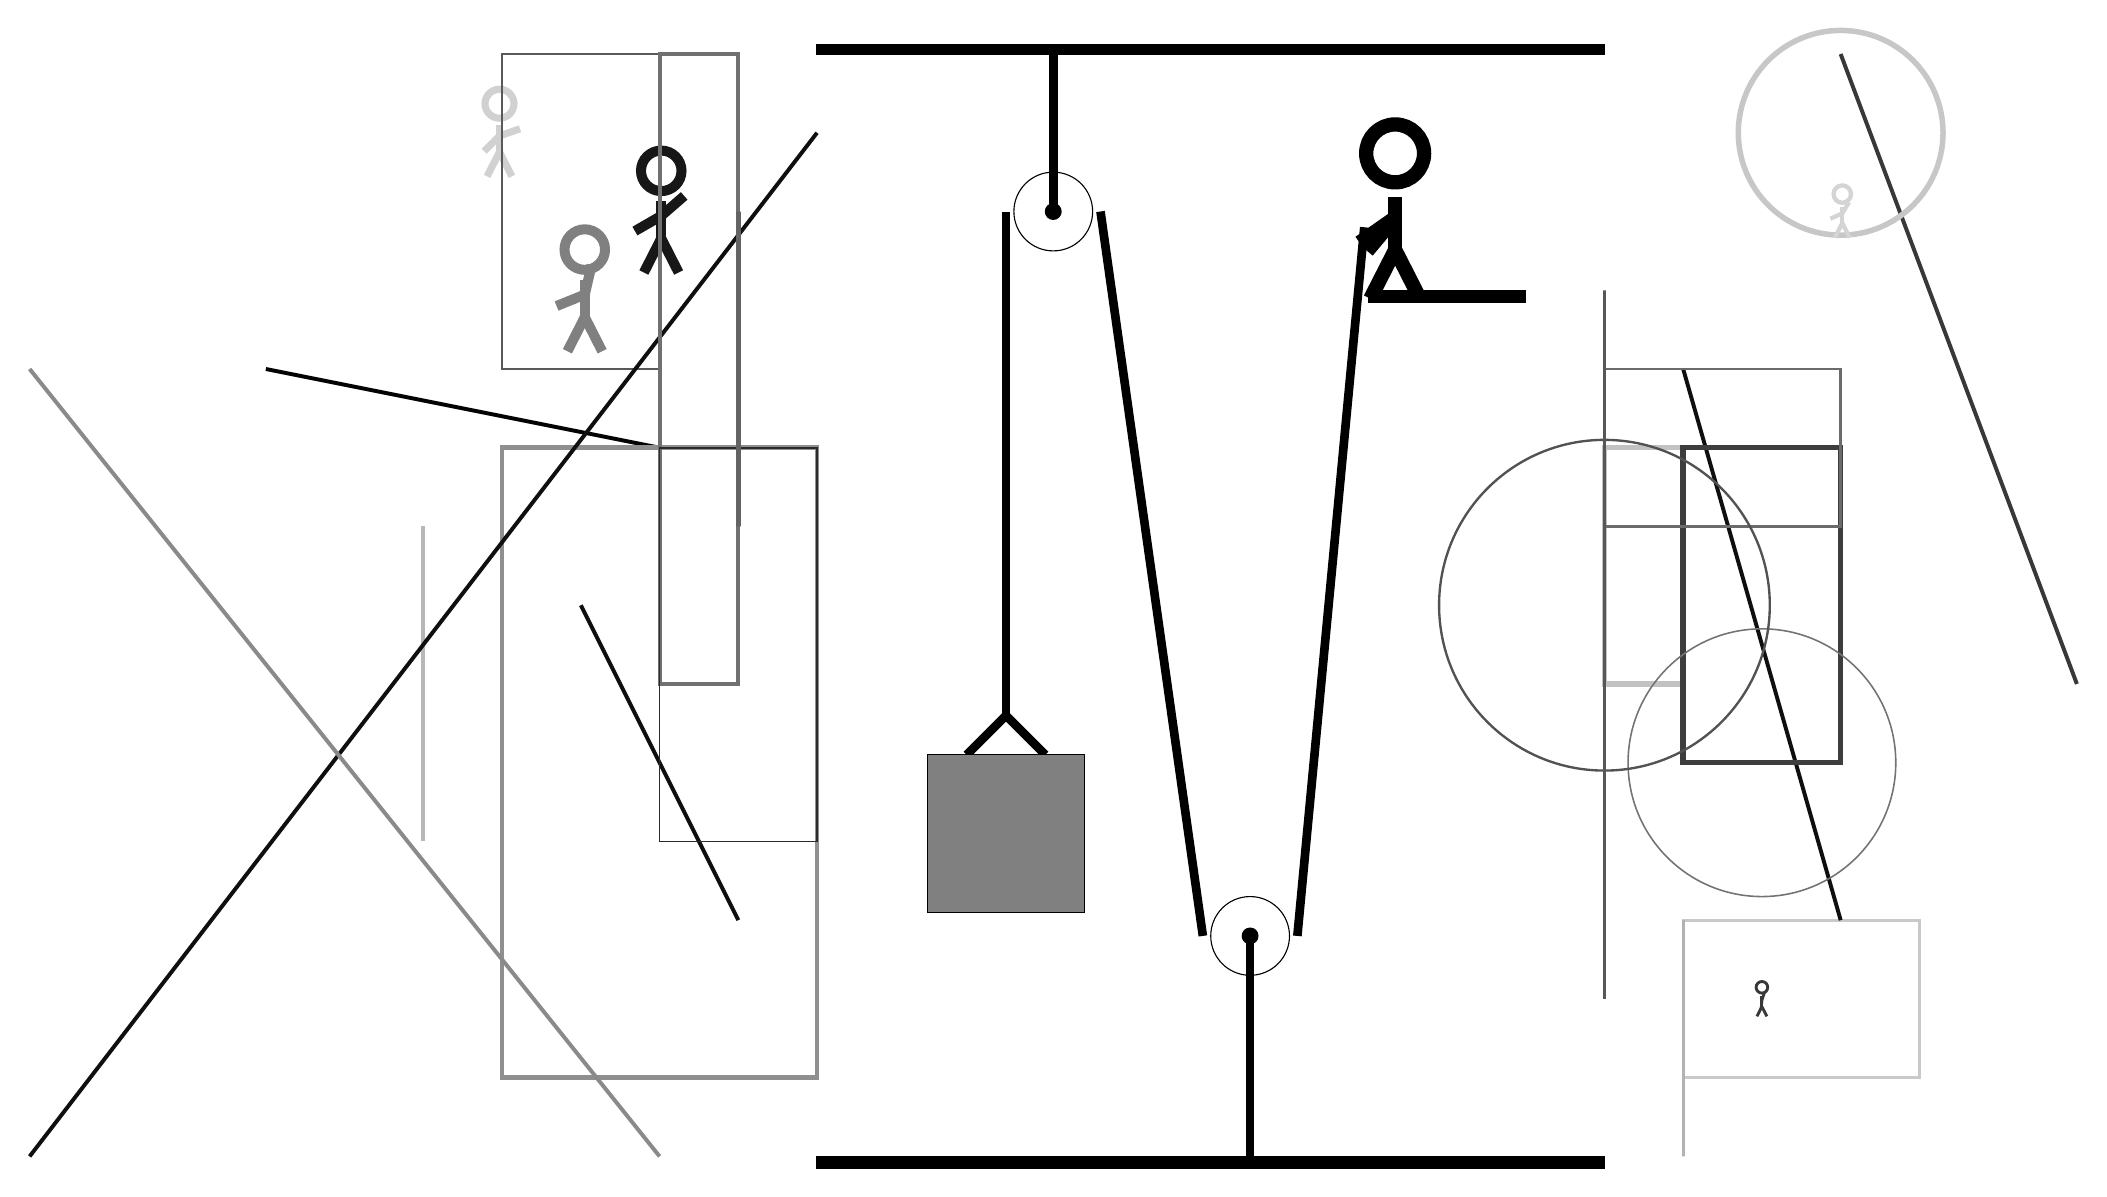
\begin{tikzpicture}
			%%%%% START %%%%%
			
			\draw[fill=black] (-2, 14) rectangle (8, 14.125);
			
			\draw (3.5, 2.8) circle (0.5);
			\draw[fill=black] (3.5, 2.8) circle (0.1);
			\draw[line width=1.1mm] (3.5, 2.8) -- (3.5, 0);
			
			\draw (1, 12) circle (0.5);
			\draw[fill=black] (1, 12) circle (0.1);
			\draw[line width=1.1mm] (1, 14) -- (1, 12);
			
			\draw[line width=1.1mm](-0.1, 5.1) --  (0.4, 5.6) -- (0.9, 5.1);
			\draw[fill=black!50] (-0.6, 5.1) rectangle (1.4, 3.1);
			
			\draw[line width=1.1mm](0.4, 12) -- (0.4, 5.6);
			\centerarc[line width=1.1mm](1, 12)(180:0:0.6)
			\draw[line width=1.1mm](1.6, 12) -- (2.9, 2.8);
			\centerarc[line width=1.1mm](3.5, 2.8)(180:360:0.6)
			\draw[line width=1.1mm](4.1, 2.8) -- (4.95, 11.8);
			
			\node at (5.3, 12) {\Strichmaxerl[10][35][-130]};
			\draw[fill=black] (5, 11) rectangle (7, 10.85);
			
			\draw[line width=0.7mm, color=black!24] (8, 9) rectangle (9, 6);
			
			\draw[line width=0.4mm, color=black!21] (9, 3) rectangle (12, 1);
			\draw[line width=0.4mm, color=black!30] (9, 3) rectangle (9, 0);
			\node[line width=0.5mm, color=black!91] at (-4, 12) {\Strichmaxerl[7][30][41]};
			\draw[line width=0.5mm, color=black!94](-5, 7) -- (-3, 3);
			\draw[line width=0.5mm, color=black!78](11, 14) -- (14, 6);
			
			\node[line width=0.4mm, color=black!78] at (10, 2) {\Strichmaxerl[2][85][72]};
			
			\draw[line width=0.5mm, color=black!94](9, 10) -- (11, 3);
			\node[line width=0.3mm, color=black!18] at (-6, 13) {\Strichmaxerl[5][45][19]};
			\draw [line width=0.7mm, color=black!22](11, 13) circle (1.3);
			\draw[line width=0.5mm, color=black!99](-4, 9) -- (-9, 10);
			\draw[line width=0.6mm, color=black!44] (-2, 9) rectangle (-6, 1);
			\draw[line width=0.5mm, color=black!28](-7, 4) -- (-7, 8);
			
			\draw[line width=0.7mm, color=black!76] (9, 5) rectangle (11, 9);
			\draw[line width=0.3mm, color=black!58] (8, 10) rectangle (11, 8);
			\node[line width=0.2mm, color=black!50] at (-5, 11) {\Strichmaxerl[7][22][77]};
			
			\draw [line width=0.5mm, color=black!89](-8, 7) circle (0.0);
			\draw[line width=0.3mm, color=black!65] (-4, 10) rectangle (-6, 14);
			\draw[line width=0.5mm, color=black!94](-2, 13) -- (-12, 0);
			
			\draw[line width=0.5mm, color=black!56] (-3, 14) rectangle (-4, 6);
			\draw[line width=0.2mm, color=black!83] (-2, 9) rectangle (-4, 4);
			
			\draw[line width=0.6mm, color=black!61] (-3, 8) rectangle (-3, 12);
			\node[line width=0.2mm, color=black!17] at (11, 12) {\Strichmaxerl[3][24][59]};
			\draw [line width=0.2mm, color=black!55](10, 5) circle (1.7);
			\draw [line width=0.3mm, color=black!68](8, 7) circle (2.1);
			\draw[line width=0.3mm, color=black!66] (8, 11) rectangle (8, 2);
			\draw[line width=0.5mm, color=black!46](-4, 0) -- (-12, 10);
			
			\draw[fill=black] (-2, 0) rectangle (8, -0.15);
			
			%%%%% END %%%%%
		\end{tikzpicture}
	\end{figure}	
\end{document}